%%  Technical Chapters

\chapter{System Overview}

This project builds a system that uses EEG signals recorded from the scalp to do two
things. The first is to tell whether a person is imagining a movement of the left hand or
the right hand. The second is to find out the mental condition of the person at that
moment. Both outputs come from the same recording. The system takes the raw brain signals,
cleans them, pulls out useful information from them, and then uses a machine learning
model for the left versus right decision and a set of frequency band calculations for the
cognitive score. No audio is recorded at any stage.\\

\begin{figure}[h]
    \centering
    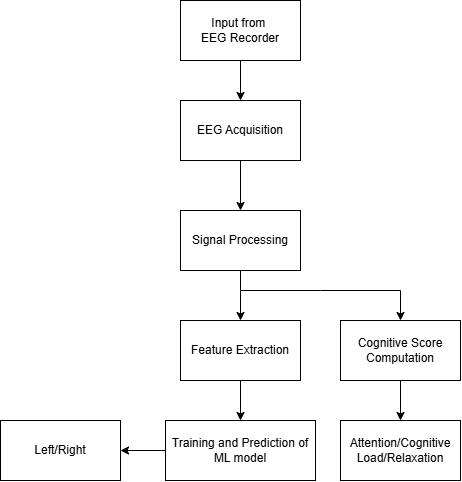
\includegraphics[width=0.60\textwidth]{BDeeg.png}
    \caption{EEG Based Cognitive Assessment Overview}
    \label{fig:system_overview}
\end{figure}

Figure~\ref{fig:system_overview} illustrates the overall architecture of the proposed
system. The first step is collecting the data. The person wears an EEG headset with
electrodes placed on the scalp at standard positions. During the recording session the
person is shown an instruction and is asked to imagine gripping an object with the left
hand or the right hand, while the EEG signals are being recorded. The task is only
imagined, so no actual movement is made and no sound is produced. To know which task was
being performed at each point in the recording, markers are placed in the recording
software at the start of every trial. These markers are what label the data, and they
replace the need for any audio reference.

The filtered EEG is then sent to the band analysis stage. Here the signal is divided into
the standard frequency bands, which are delta, theta, alpha, beta and gamma, to study the
brain activity. The bands matter for both halves of the system. For motor imagery, the
alpha and beta bands over the motor cortex are the ones that change when a movement is
imagined. For the cognitive score, the balance of power between the bands is what
indicates whether the person is attentive, under load, relaxed, stressed or tired.

The next step is feature extraction, which means taking out useful information from the
EEG signals. For the motor imagery path, the two motor cortex channels C3 and C4 are
filtered to the 8--30 Hz range, their power is computed, and the change in power with
respect to a baseline taken just before the task is calculated. Statistical measures such
as the mean, median, skewness and kurtosis of each channel are then worked out, along with
the ratio of power between C3 and C4 and the band power over 8--30 Hz. These values
together form a set of numbers that represent what the motor cortex was doing during that
trial. For the cognitive path, the power spectral density is computed and the relative
power in each band is obtained by dividing the power in that band by the total power.

The machine learning model is trained using the features extracted from the EEG data along
with the labels that say whether the trial was a left-hand or a right-hand imagination. The
model looks at the patterns in the features and tries to learn which pattern belongs to
which side. Once training is done, the model can take a new EEG trial and predict whether
the person imagined the left or the right hand. In parallel, the relative band powers are
combined into ratios to produce the cognitive outputs, which are attention, cognitive load,
relaxation, stress and fatigue.

The output of the system is therefore the predicted side, left or right, along with the
cognitive score. The predicted side shows which hand the person was imagining, and the
cognitive score shows how attentive, stressed or tired the person is at that moment. Both
outputs come from the same EEG recording setup, which keeps the system simple and practical
to use.

Overall this system takes EEG signals as input, processes them, and uses machine learning
and frequency band analysis to give two useful outputs. It works with a simple wearable
headset and needs nothing besides the EEG signal itself, which makes it a practical
approach for real world use.

%% new chapter

\chapter{System Hardware}
This chapter goes through the hardware used in the project and why each part was picked.
There are four main parts: the GELO headset that picks up the EEG, the Raspberry Pi 5 that
is meant to run the processing, a metal case with fans that keeps the Pi cool, and a small
touch screen that shows the interface. The EEG recorder is covered first, since the choice
of recorder decides most of what the rest of the system can do.

\section{EEG Recorder}
An EEG recorder is a device that measures the tiny voltages on the scalp through a set of
electrodes and sends them to a computer. Recorders differ in how many electrodes they
have, how the electrodes touch the skin, how comfortable they are, and whether they need a
cable. The two main families are described below.

\subsection{Wet Electrode EEG System}

In a wet system a gel or saline solution is put between each electrode and the skin. The
liquid lowers the contact resistance, so the recorded signal is clean and steady. This is
why hospitals and research labs use wet caps, usually with the electrodes laid out
according to the international 10--20 placement scheme \cite{jasper1958tentwenty}, which
names each position by its distance from fixed points on the skull.

For this project a wet system was not a good fit. Putting gel on every electrode takes
time before each session, the gel dries out over a long recording, the hair has to be
washed afterwards, and the cap itself needs cleaning. All of this goes against the aim of
a headset that a person can put on and use in daily life without help.

\subsection{Dry Electrode EEG System}

A dry system presses the electrodes directly against the skin with no gel at all. Setup
takes a minute or two, the person can wear the device without help, and nothing needs
cleaning afterwards. The trade-off is a higher contact resistance, so the signal is
somewhat noisier and more sensitive to movement. Dry electrodes appear in several shapes
of device, such as headbands and headphones. A headphone design was chosen here, because
it sits firmly over the ears and the top of the head, where the motor cortex electrodes
need to be, and it is comfortable for longer sessions. This led to the GELO BCI headset.

\subsection{GELO BCI Headset}
The GELO BCI headset, shown in Figure~\ref{fig:gelo}, looks and works like an ordinary pair
of wireless headphones, but it has dry electrodes built into the headband and ear cups.
It records four EEG channels, named A1, A2, C3 and C4, against a reference electrode at Cz,
with two further electrodes acting as ground. The names follow the 10--20 scheme
\cite{gelo2026manual}.

These positions are the main reason the device suits this project. C3 lies over the left
motor cortex and C4 over the right, and these are the two places where the activity
changes when a person imagines moving a hand, so they carry the information needed for the
left and right decision. A1 and A2 sit on the ears, where there is very little brain
activity. Each motor channel is read against its ear electrode, as A1--C3 and A2--C4, so
that noise reaching both electrodes of a pair is largely cancelled. All four channels are
also used for the band powers behind the cognitive score.

The headset samples each channel 250 times a second, which is more than enough for the
0.5--35 Hz range studied here, and sends the data over Bluetooth Low Energy, so the
person is not tied to the computer by a cable. Since it is also a pair of headphones, it
has speakers and a microphone. Neither is used in this work, as no sound is recorded, but
the speakers could later play an audio cue at the start of each trial. The main
specifications are listed in Table~\ref{tab:gelo_spec}.

\begin{table}[!htbp]
\centering
\caption{Main specifications of the GELO BCI headset \cite{gelo2026manual}}
\label{tab:gelo_spec}
\begin{tabular}{|l|l|}
\hline
\textbf{Item} & \textbf{Value} \\
\hline
EEG channels & 4 (A1, A2, C3, C4) \\
\hline
Reference and ground & Cz reference, two ground electrodes \\
\hline
Electrode type & Dry, gold-plated spring pins \\
\hline
Sampling rate & 250 Hz per channel \\
\hline
Read mode & Bipolar (A1--C3, A2--C4) \\
\hline
Wireless link & Bluetooth Low Energy 5.0 \\
\hline
Audio & Two 40 mm speakers, 20 Hz -- 20 kHz \\
\hline
Bluetooth audio profiles & HFP, HSP, A2DP \\
\hline
\end{tabular}
\end{table}

\begin{figure}[!htbp]
    \centering
    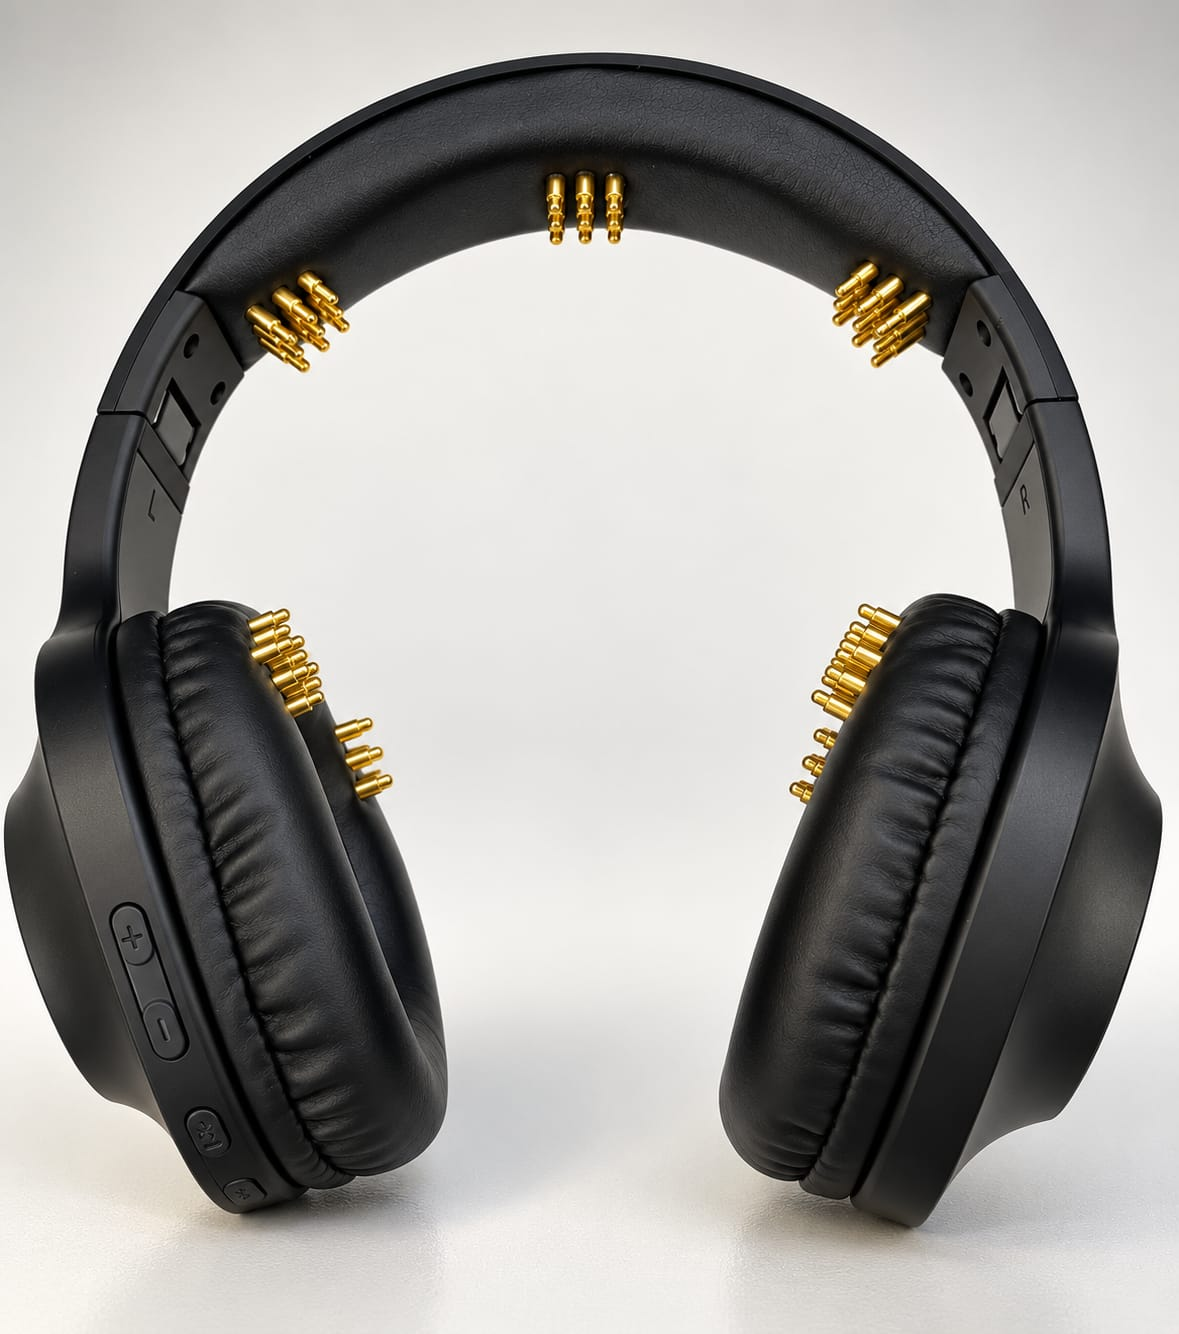
\includegraphics[width=0.65\linewidth]{Pic1.jpeg}
    \caption{GELO BCI Headset}
    \label{fig:gelo}
\end{figure}

\newpage

\section{Raspberry Pi 5}

The Raspberry Pi 5, shown in Figure~\ref{fig:rpi5}, is the small computer chosen to run
the whole system on its own once development is finished. Its job is to receive the EEG
from the headset over Bluetooth, filter it, compute the features, run the classifier and
the cognitive score, and draw the interface on the screen.

At its heart is a Broadcom BCM2712 chip with four Arm Cortex-A76 cores running at up to
2.4 GHz \cite{rpi5brief}. The processing in this project is light by modern standards: a
few filters, a Welch spectrum and a linear SVM on a handful of features every fraction of
a second, so this processor has plenty of headroom. The board has Bluetooth built in,
which is how the headset connects, along with Wi-Fi, Ethernet, USB 3.0 ports and two
micro-HDMI outputs, one of which drives the display. The 40-pin header can be used later
to send the left or right decision to a motor driver or a robot. Its main specifications
are given in Table~\ref{tab:rpi_spec}.

\begin{table}[!htbp]
\centering
\caption{Main specifications of the Raspberry Pi 5 relevant to this project \cite{rpi5brief}}
\label{tab:rpi_spec}
\begin{tabular}{|l|l|}
\hline
\textbf{Item} & \textbf{Value} \\
\hline
Processor & Broadcom BCM2712, 4 $\times$ Cortex-A76, 2.4 GHz \\
\hline
Memory & 4 GB or 8 GB LPDDR4X \\
\hline
Wireless & Wi-Fi (2.4 and 5 GHz), Bluetooth 5.0 / BLE \\
\hline
Wired & Gigabit Ethernet, 2 $\times$ USB 3.0, 2 $\times$ USB 2.0 \\
\hline
Display output & 2 $\times$ micro-HDMI \\
\hline
Expansion & 40-pin GPIO header, PCIe 2.0 $\times$1 \\
\hline
Other & Real-time clock, power button \\
\hline
\end{tabular}
\end{table}

\begin{figure}[!htbp]
    \centering
    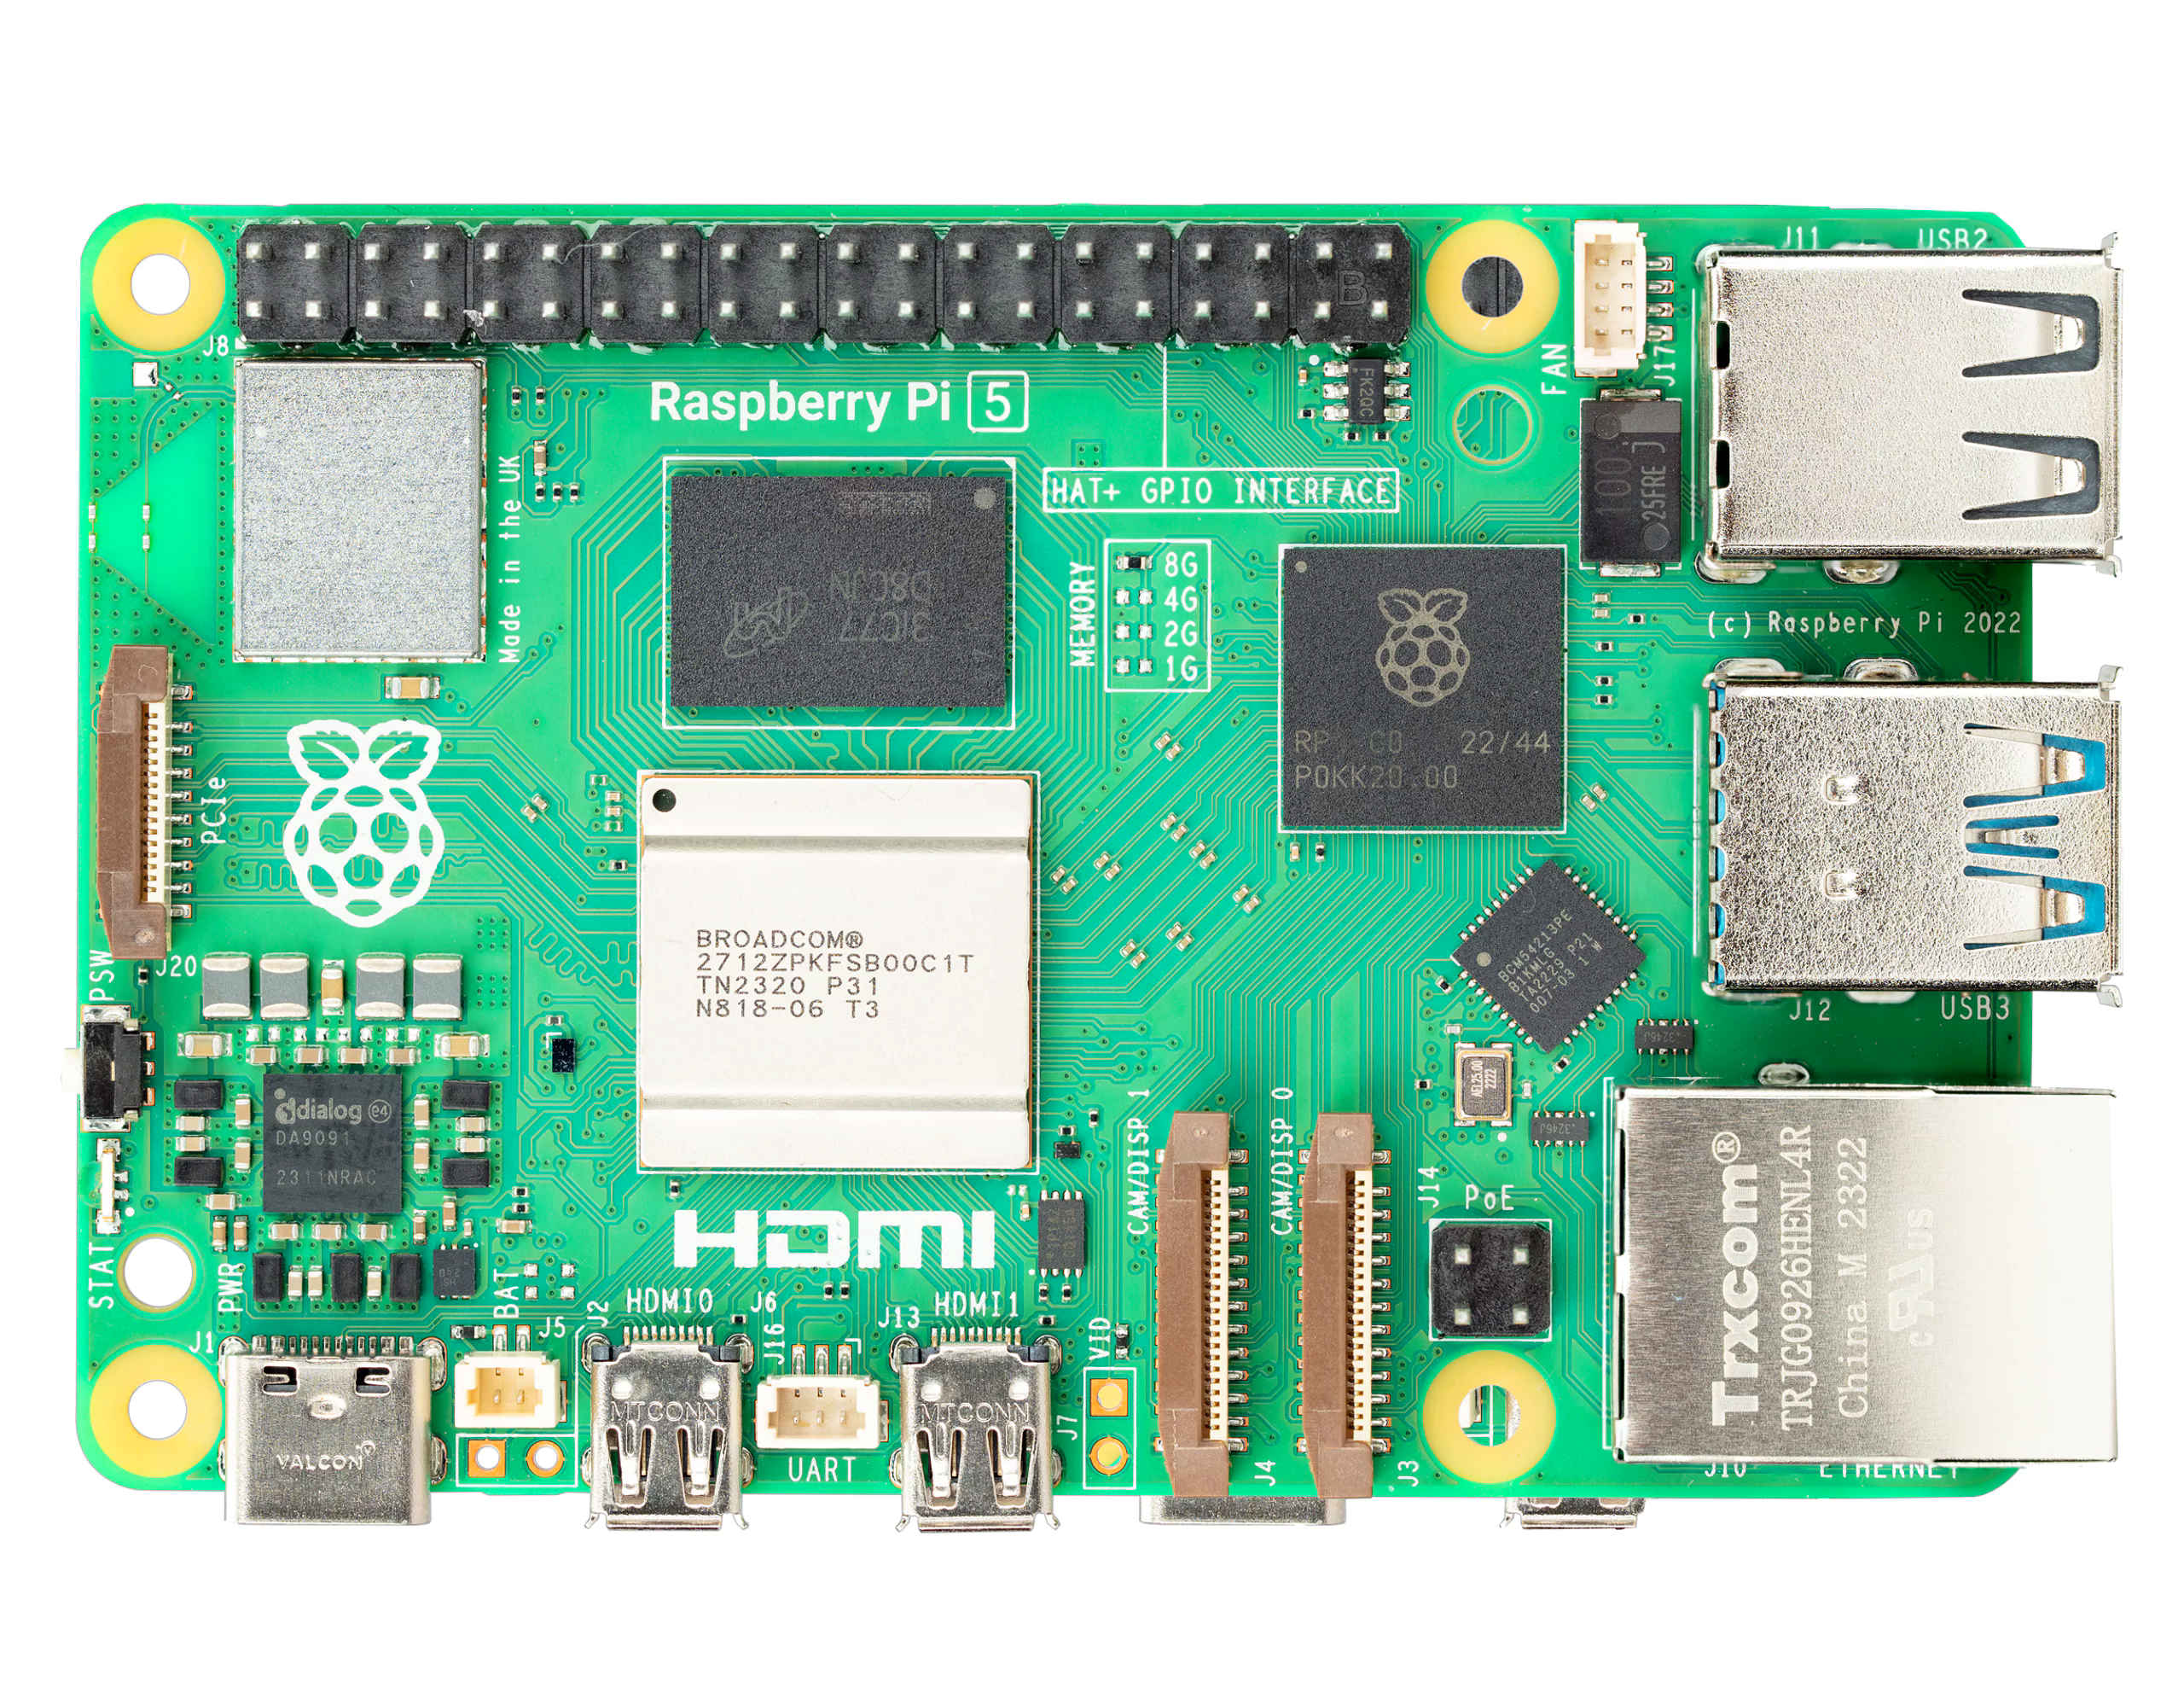
\includegraphics[width=0.65\linewidth]{pi.jpg}
    \caption{Raspberry Pi 5}
    \label{fig:rpi5}
\end{figure}

\newpage

\section{Aluminum Heat Sink Case with Dual Fans for Raspberry Pi 5}

The Raspberry Pi 5 gets hot when it works without a break, and once its temperature passes
a set limit it slows its own clock to protect itself. For a system that has to process
EEG continuously for a whole session, that slowdown would make the output lag. The case
shown in Figure~\ref{fig:heatsink} prevents this.

The case is machined from aluminium, a metal that conducts heat very well, so the whole
body of the case acts as one large heat sink that draws heat away from the chip. Two small fans on top
blow air across it to remove that heat faster. The metal body also shields the board from
knocks and dust, which matters because the unit is meant to be carried around with the
headset rather than sit on a lab bench.

\subsection{Features of Aluminum Heat Sink}

\begin{itemize}
    \item The aluminium body itself works as a large passive heat sink
    \item Two fans add airflow when the processor is under steady load
    \item Keeps the Pi below the temperature at which it slows down
    \item Gives the board a solid, closed housing for portable use
\end{itemize}

\begin{figure}[!htbp]
    \centering
    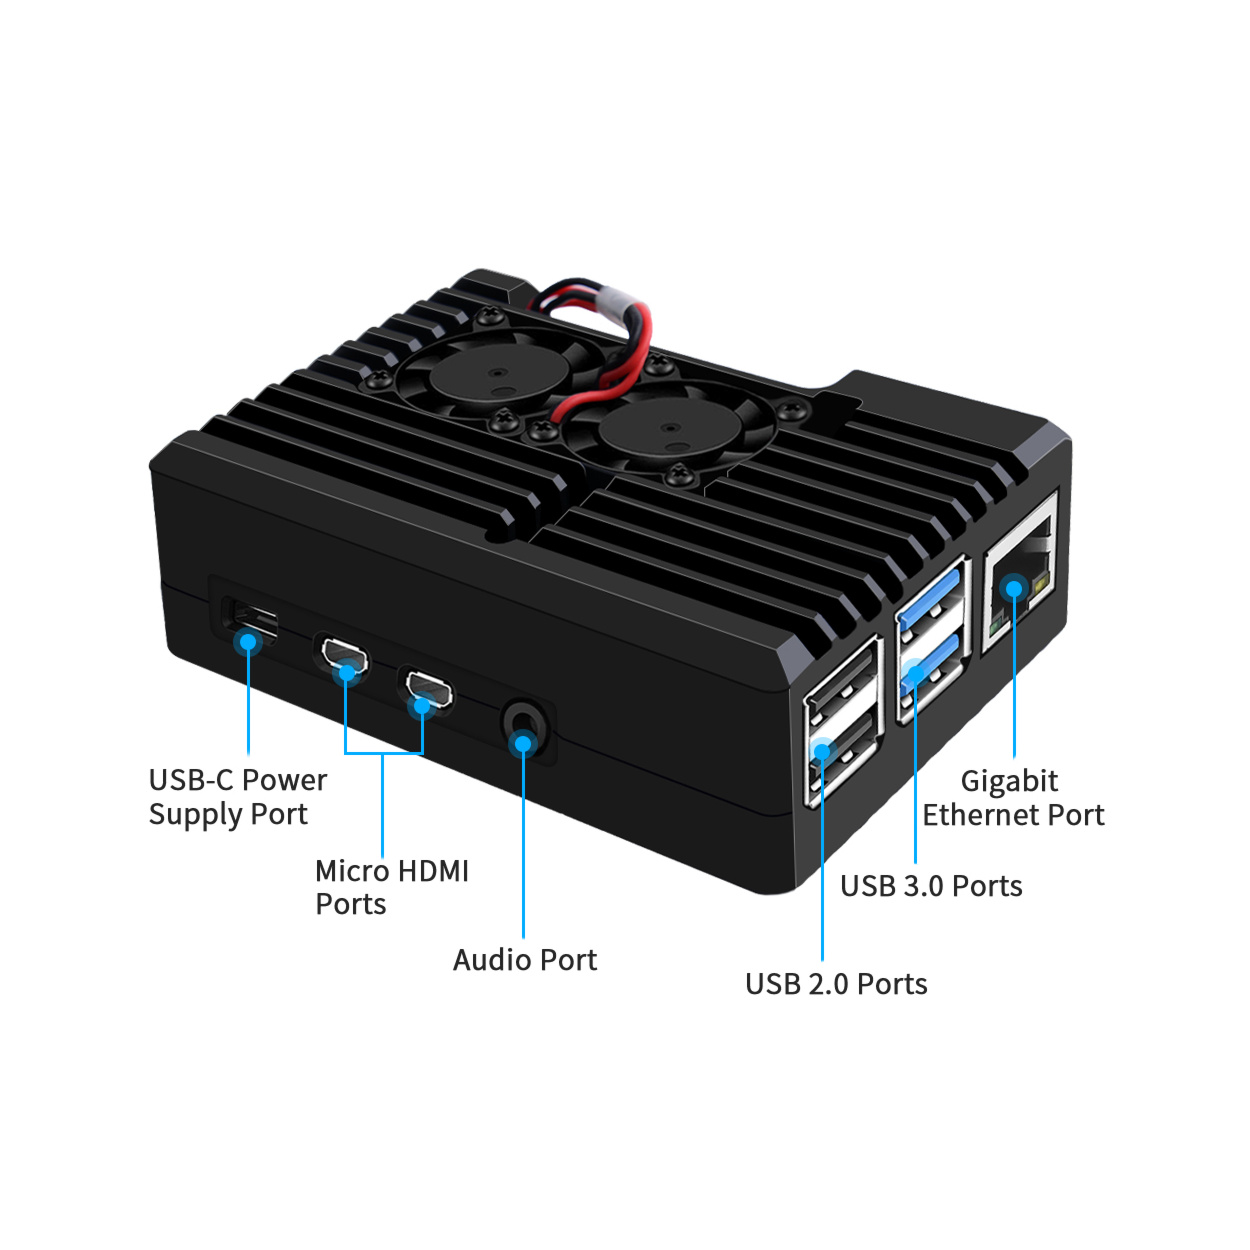
\includegraphics[width=0.55\linewidth]{sfs_03_2.jpg}
    \caption{Aluminum Heat Sink Case with Dual Fans for Raspberry Pi 5}
    \label{fig:heatsink}
\end{figure}

\section{Waveshare 7-Inch LCD Display}

The 7-inch Waveshare touch screen \cite{waveshare7inch}, shown in Figure~\ref{fig:lcd}, is
how the person using the system sees what is going on. During a recording it shows the
left and right arrows the subject has to follow, the live EEG traces, and the status of
the electrodes. After processing it shows the predicted side and the cognitive scores.

The screen connects to the Raspberry Pi through HDMI for the picture and USB for the touch
input, and it is supported by Raspberry Pi OS. Because it is a touch
screen, the session can be started, calibrated and stopped with a finger, so no keyboard or
mouse is needed. Its small size keeps the whole set-up portable, which is useful for
demonstrations and for recording outside the lab.

\subsection{Features of Waveshare LCD Display}
\begin{itemize}
    \item 7-inch screen, large enough to read the scores from a normal distance
    \item HDMI picture input and USB touch input, both supported by the Pi
    \item Touch control, so no keyboard or mouse is needed during a session
    \item Light and compact, so the system can be carried with the headset
\end{itemize}

\begin{figure}[!htbp]
    \centering
    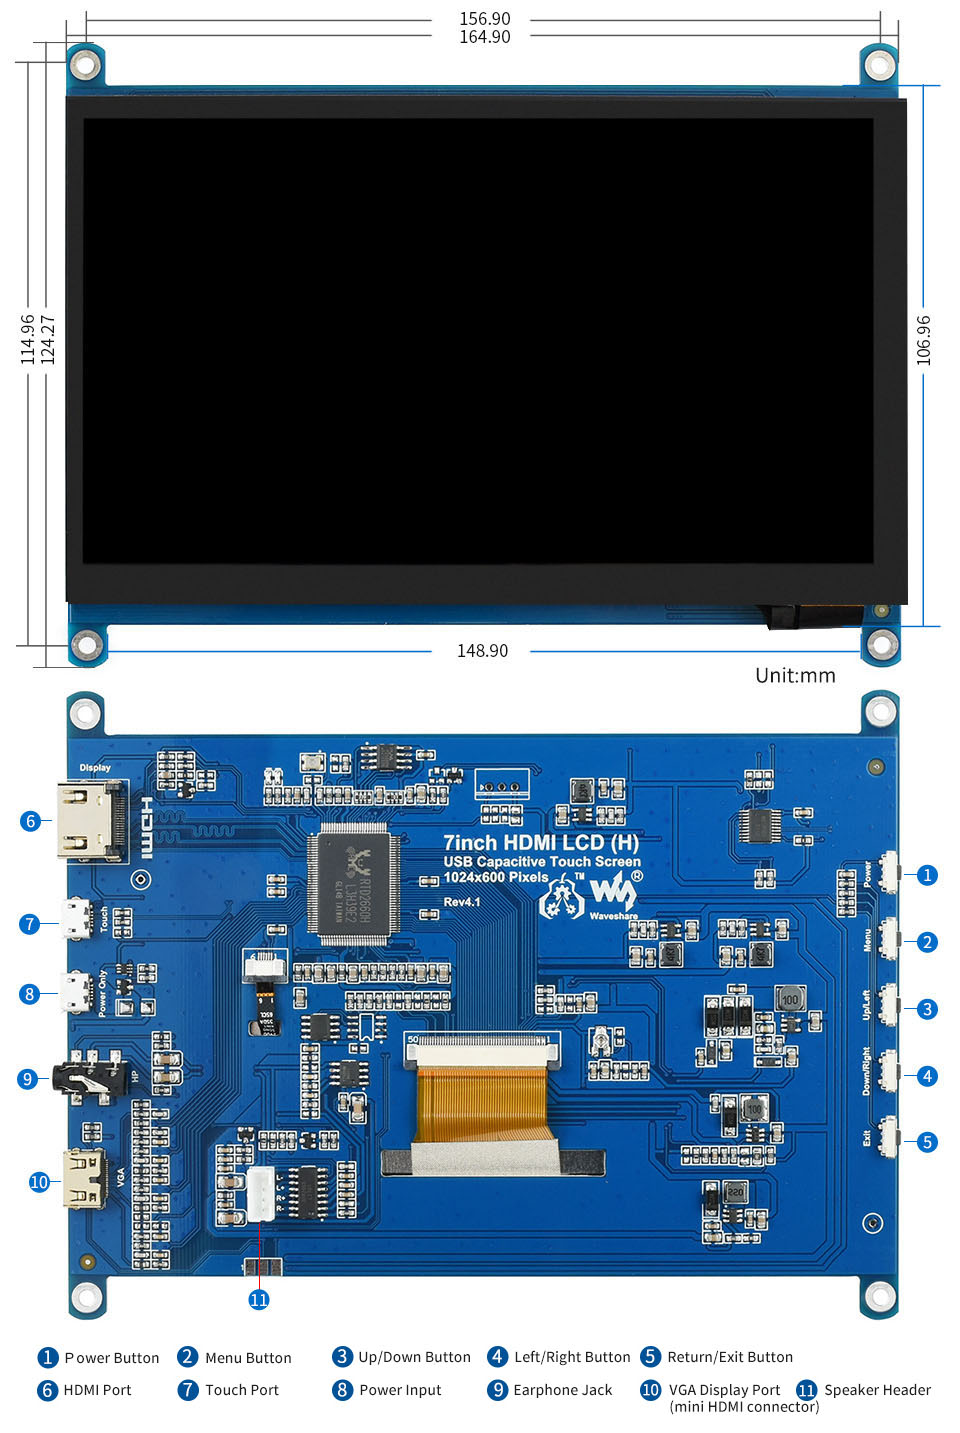
\includegraphics[width=0.55\linewidth]{Exterior-Size.jpg}
    \caption{Waveshare 7-Inch LCD Display}
    \label{fig:lcd}
\end{figure}

\chapter{System Software}

This chapter explains the software setup used to develop the proposed EEG-based motor
imagery classification and cognitive assessment system. It includes the software
environment, the GUI software, the EEG signal collection process, and the libraries used
for signal processing, visualization, machine learning and cognitive score calculation. The
system combines real-time EEG data collection using the Capsule GUI with Python-based
preprocessing and classification methods to perform EEG signal analysis in a reliable way.

\section{Software Requirements}

The proposed system uses the Capsule GUI software for real-time EEG signal acquisition,
electrode impedance checking, calibration, signal display and marker placement. All
recording and processing reported in this work is carried out on a Windows 11 computer. The
Raspberry Pi 5 described in the previous chapter is the intended deployment platform, so
that the complete system can later run as a standalone unit, but the results presented in
this report were obtained on the Windows setup.

The recording and analysis set-up is summarised in Table~\ref{tab:sw_setup}, and the
Python libraries, with the job each one does in this project, are listed in
Table~\ref{tab:sw_libs}.

\begin{table}[!htbp]
\centering
\caption{Software set-up used in this project}
\label{tab:sw_setup}
\begin{tabular}{|l|p{10cm}|}
\hline
\textbf{Item} & \textbf{Used for} \\
\hline
Windows 11 & All recording and analysis reported here \\
\hline
Raspberry Pi OS & Planned stand-alone version of the system \\
\hline
Capsule GUI & Connecting the headset, checking electrode resistance, calibration, live view, placing trial markers \\
\hline
Python 3 & Conversion of recordings, feature calculation, SVM training, cognitive score and the application window \\
\hline
MATLAB & ERD/ERS and PSD of the stroke and BCI Competition IV 2b datasets, the ERD\% SVM on the 2b data (\texttt{fitcsvm}) and the report figures \\
\hline
\end{tabular}
\end{table}

\begin{table}[!htbp]
\centering
\caption{Python libraries and what each one does in this project}
\label{tab:sw_libs}
\begin{tabular}{|l|p{10cm}|}
\hline
\textbf{Library} & \textbf{Job in this project} \\
\hline
NumPy & Holds the EEG samples as arrays; sums spectrum bins into bands; computes the ratios \\
\hline
SciPy & Butterworth band-pass and notch filters, Welch spectra \\
\hline
Pandas & Reads the CSV files and keeps track of which trial belongs to which hand \\
\hline
h5py & Opens the \texttt{.h5} files saved by the Capsule software \\
\hline
MNE-Python \cite{gramfort2013mne} & Channel handling and cutting the recording into trials around each marker \\
\hline
Scikit-learn \cite{pedregosa2011sklearn} & Feature scaling, SVM training and accuracy checks \\
\hline
Matplotlib & Static plots: PSD, ERD curves, band bars and the figures in this report \\
\hline
PyQtGraph & Fast-refreshing live EEG trace during a session \\
\hline
CustomTkinter & The application window: sidebar, cards, buttons and dialogs \\
\hline
PyTorch (optional) & Kept for possible deep learning models later \\
\hline
\end{tabular}
\end{table}

Two plotting libraries are used on purpose. Matplotlib gives neat static figures for
analysis and for this report, but it is slow to redraw, so the live trace that has to
update many times a second is drawn with PyQtGraph instead.

\vspace{0.5cm}

\section{Flowchart}
The system shown in Figure~\ref{fig:Flowchart} starts with the person putting on the EEG
headset and the headset being paired with the computer over Bluetooth. The resistance of
each of the four electrodes is then checked, since a poor contact makes the rest of the
recording useless. Two short calibration steps follow. In the first, the subject keeps the
eyes closed for 30 seconds so that the individual alpha peak frequency can be found, as
alpha activity is strongest with the eyes closed. In the second, the subject looks at a
fixed point for 30 seconds so that the median power in each frequency band can be stored
as a baseline. Later readings are compared against this baseline rather than against fixed
values, which makes the scores specific to that person.

\begin{figure}[!htbp]
    \centering
    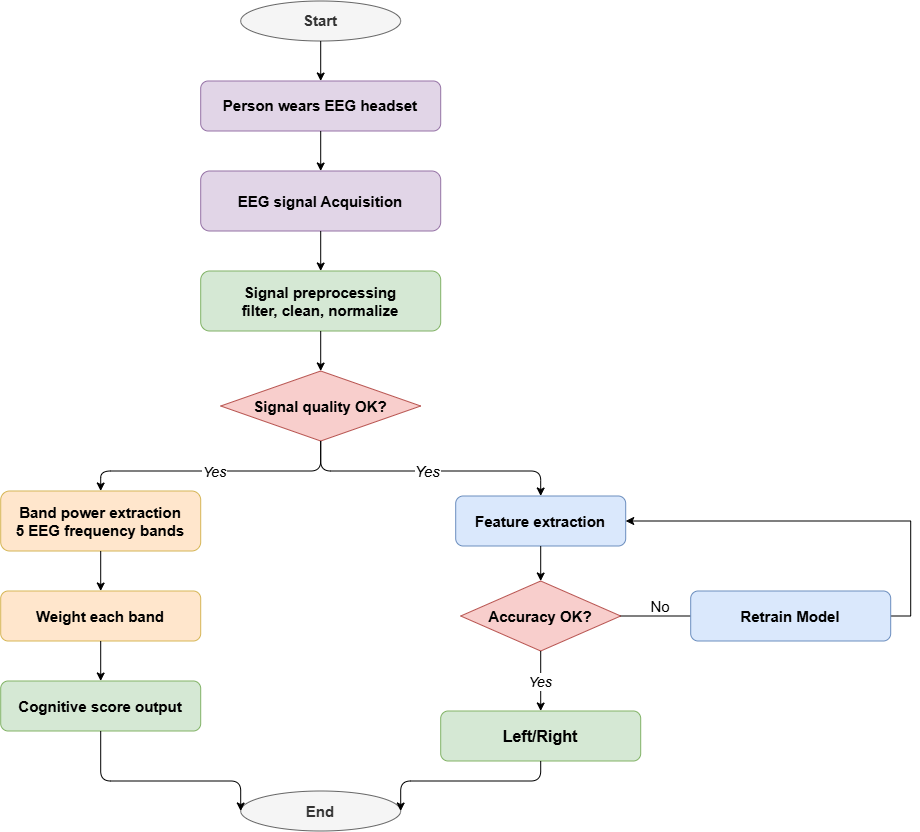
\includegraphics[width=1\linewidth]{flowchart_1.png}
    \caption{Flowchart of EEG based Cognitive Assessment Model}
    \label{fig:Flowchart}
\end{figure}
\newpage

\FloatBarrier

Once calibration is complete, the recording begins and the subject performs the motor
imagery trials. A marker is placed at the start of each trial so that every segment of the
recording is tied to a known label, either left-hand or right-hand imagination. The session
is then saved in \texttt{.h5} format and converted to CSV using a Python script for further
analysis. No audio is recorded at any point.

If the signal is too noisy or unclear, the recording is done again from the beginning. Only
when the signal quality is good enough does the system move forward. After passing the
quality check, the pipeline splits into two separate paths that run independently.

The first path handles cognitive assessment. Here the EEG signal is broken down into the
five frequency bands, which are delta, theta, alpha, beta and gamma. The power of each band
is calculated and divided by the total power to give its relative power, which removes the
effect of the overall signal level changing as electrode contact improves or worsens. These
relative powers are then combined into ratios to give the cognitive outputs. Attention,
cognitive load and relaxation are read from the device SDK, while stress is obtained from
the ratio of relative high-beta power to relative alpha power, and fatigue from the ratio
of combined theta and alpha power to beta power. Each ratio is compared against the
person's own reference value and mapped onto a score between 0 and 100, so the result tells
how mentally active or tired the person is at that moment.

The second path handles motor imagery classification. In this path the C3 and C4 channels
are taken out and filtered to the 8--30 Hz band, a fixed window of 4 seconds is cut from
the start of each imagination, and the power and the change in power relative to the
baseline are computed. Features such as the mean, median, skewness and kurtosis of each
channel, the ratio of power between C3 and C4, and the band power over 8--30 Hz are then
extracted. These features are used to train a Support Vector Machine. After training, the
model accuracy is checked. If the accuracy is not satisfactory, the process goes back to
the feature extraction stage, the feature set or the kernel is adjusted, and the model is
retrained. This loop continues until the accuracy reaches an acceptable level. Once the
accuracy is good, the model is used to predict left or right from new EEG recordings.

Both paths finish at the end node, giving two outputs from a single EEG recording setup,
which are the cognitive score and the predicted side.